\documentclass{beamer}
\usepackage[T1]{fontenc}
\usepackage[utf8]{inputenc}
\usepackage{amsfonts}
\usepackage{lmodern}
\usepackage{graphicx} 
\usepackage{color}
\usepackage{attrib}
\usepackage{ragged2e}
\usepackage{algorithm2e}

\setcounter{secnumdepth}{3}
\setcounter{tocdepth}{3}

\addtobeamertemplate{block begin}{}{\justifying}

\begin{document}

%% Spread
\newcommand{\Spt}{\ensuremath{Sp_{t}}}

\newcommand{\MSpc}{\ensuremath{Sp_{t|t-1}}}
\newcommand{\MSpn}{\ensuremath{Sp_{t+1|t}}}
\newcommand{\MSpo}{\ensuremath{Sp_{t-1|t-1}}}

%% Czas
\newcommand{\ts}{\ensuremath{{t}} }
\newcommand{\tsl}{\ensuremath{{t-1}} }


\author{Zygmunt Zawadzki}
\institute{University of Economics in Cracow, \\


\includegraphics[height=0.5cm]{volatech.png}}

\title{Filtering outliers in High-Frequency Financial Data for algorithmic trading}

\begin{frame}
\date{The first Cracow scientific seminar on the applications of nonparametric statistics and robust statistics in economics \\ 2015-05-25}
  \titlepage
\end{frame}

\begin{frame}
\tableofcontents
\end{frame}

\begin{frame}

\section{Algorithmic trading}
\begin{block}{Algorithmic trading - definition}
Algorithmic trading attempts to eliminate the human factor from the investment process - all decisions regarding the size and direction of the portfolio positions taken are made by previously created and tested algorithms. This kind of approach allows for the analysis of a much broader range of financial instruments, and thus for a greater diversification, which has a significant effect on minimizing risk.
\end{block}

\end{frame}

\section{Outliers - overview}

\begin{frame}{Definition}

\begin{block}{}
\Large
\textbf{Outliers} are sample values that cause surprise in relation to the majority of the sample.
\vskip3mm

\hspace{50pt}\normalsize{--- W.N. Venables and B.D. Ripley. 2002. Modern applied statistics with S. New York: Springer, p.119}
\end{block}

\end{frame}

\begin{frame}{Example}

\begin{figure}
    \centering
    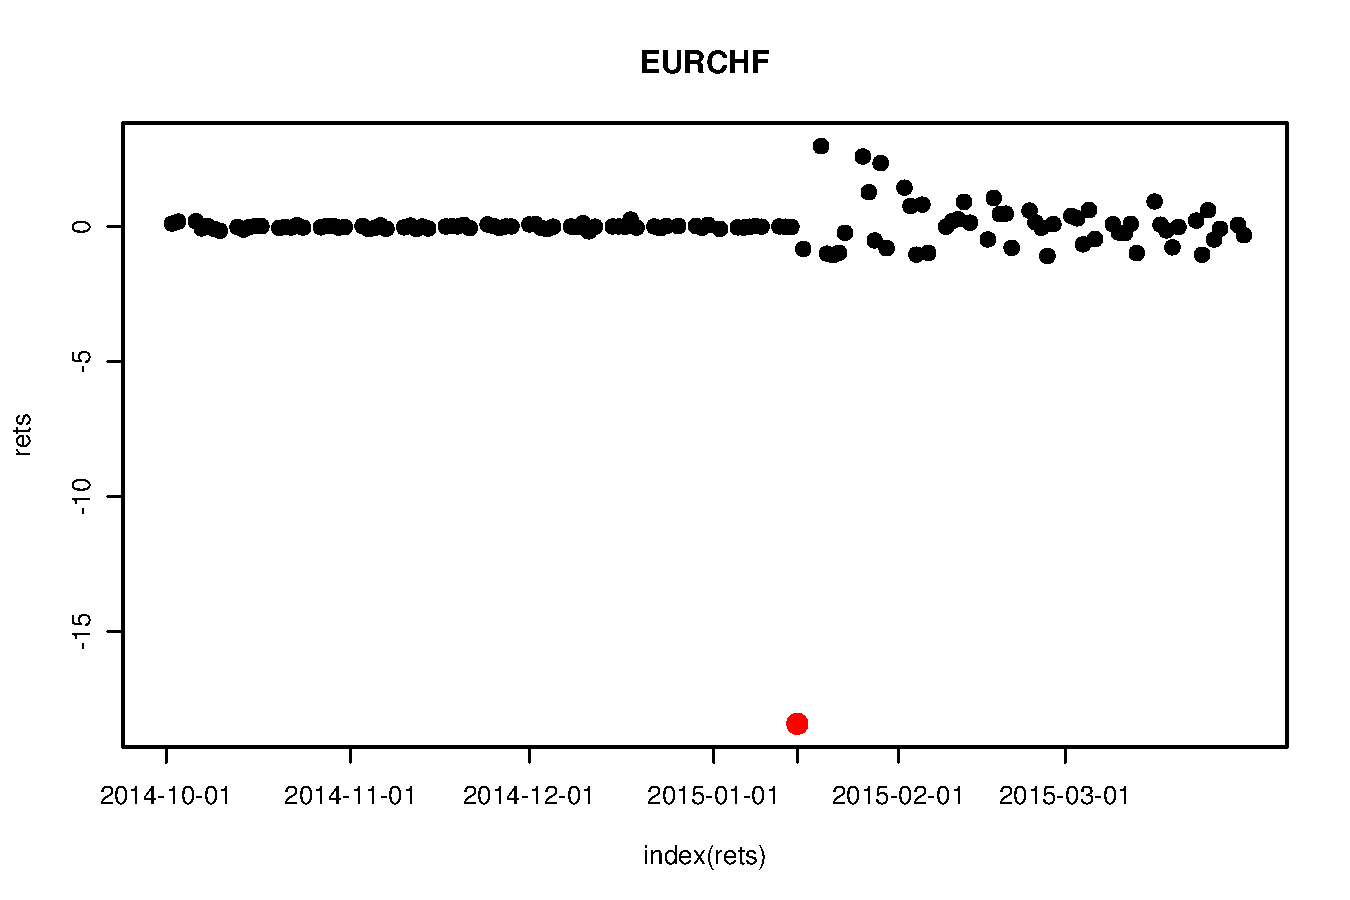
\includegraphics[width=1\textwidth]{../wykresy/EURCHF}
    \caption{Daily returns for EURCHF. There is one outlier in 2015-01-15.}
\end{figure}

\end{frame}

\begin{frame}{Potential issues}

Outliers can distort any analysis in many ways. Especially, they can disrupt indication of the volatility estimators, which are used in risk analysis. Such incident can have strong influence on weights in portfolio, and consequently disturb any diversification effect.

From statistical point of view, many classical methods are practically useless in presence of outliers (e.g. estimator's bias is to large, or we cannot control significance level in statistical test).

\end{frame}

\begin{frame}{How to handle outliers:}

\Large
\begin{itemize}
\item Use an appropriate model (e.g. techniques related to robust statistics).
\item Remove them.
\end{itemize}


\end{frame}


\section{Role of robust statistics in  algorithmic trading}
\begin{frame}{Role of robust statistics in  algorithmic trading}

Any observation for financial instrument in algorithmic trading is utilized in many ways. Firstly, it is sent to signal generator. Then this data point is passed to risk module, which calculates allowed position size based on instrument’s volatility and with relation to other portfolio constituents. If one tries to use robust methods, he must be very consistent in this choice, and use them on all these levels, starting from signal generation, through risk measures, up to measures of dependence between instruments. Any disruption from one of these elements can corrupt indication of the rest (e.g. position size for perfect signal will be dramatically reduced because of outlier that caused an increase in volatility measure used in risk analysis).

\end{frame}

\begin{frame}{Role of robust statistics in  algorithmic trading}

Methods of robust statistics are often computationally intense, and some models cannot be evaluated within a reasonable time. We should be aware, that during tests of any strategy such model should be recalculated repeatedly, often hundreds of times. this could be a serious argument against practical use of algorithms with favorable statistical properties, but large computational complexity.

\end{frame}

\begin{frame}{Removing data samples}

Removing outliers before sending them to signal generator and other parts of execution engine, seems to be an easier solution, but we have to have reliable model for financial time series. This is especially important in the presence of fat tails - in this case observation which looks unusual and could be classified as an outlier is in fact quite common and removing it would definitely change statistical properties of such time series.

\end{frame}

\section{High frequency financial data}

\begin{frame}{High frequency financial data - definition}
\small
\textbf{High frequency financial data} (HFFD) are all data related to orders, which inherently arrive at random times. Such data carry information related to any changes in order book (e.g. best bid/ask changes, execution of orders). Usually in mature markets, interval between observations is very small (Fig. \ref{fig:esh}).

\begin{figure}
    \centering
    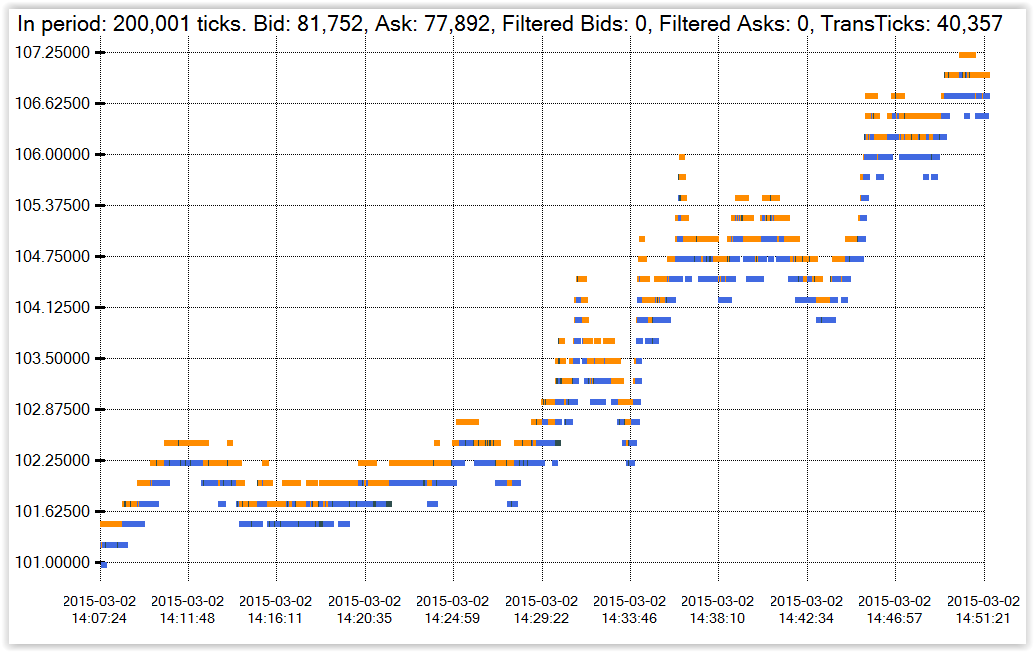
\includegraphics[width=0.6\textwidth]{../wykresy/fESH.PNG}
    \caption{There were 200 thousands changes in order book between 14:07:24, and 14:51:21 for R-Mini S\&P 500 in 2015-03-02. }
    \label{fig:esh}
\end{figure}

\end{frame}

\begin{frame}{HFFD for low frequency trading - OHLC bars}

OHLC\footnote{OHLC (Open-High-Low-Close) are created from first/highest/lowest/last observation in given interval.} bars are standard data format for most of financial analysis.


\begin{figure}
    \centering
    \includegraphics[width=.8\textwidth]{../wykresy/bpt}
    \caption{OHLC Candle plot.}
    \label{fig:esh}
\end{figure}

\end{frame}

\begin{frame}{Solution for low trading activity.}

Even when we do not operate on the highest frequency we are forced to use high frequency data to prepare reliable and evenly spaced lower frequency data. OHLC bars are usually prepared from transactions data, but for some periods, there could be no transactions at all. periods with no transaction data can be either skipped or we could use mid Bid-Ask price as a proxy.

\end{frame}

\begin{frame}{\Large OHLC bars are usually prepared from transactions data, but for some periods, there could be no transactions at all.}

\begin{figure}
    \centering
    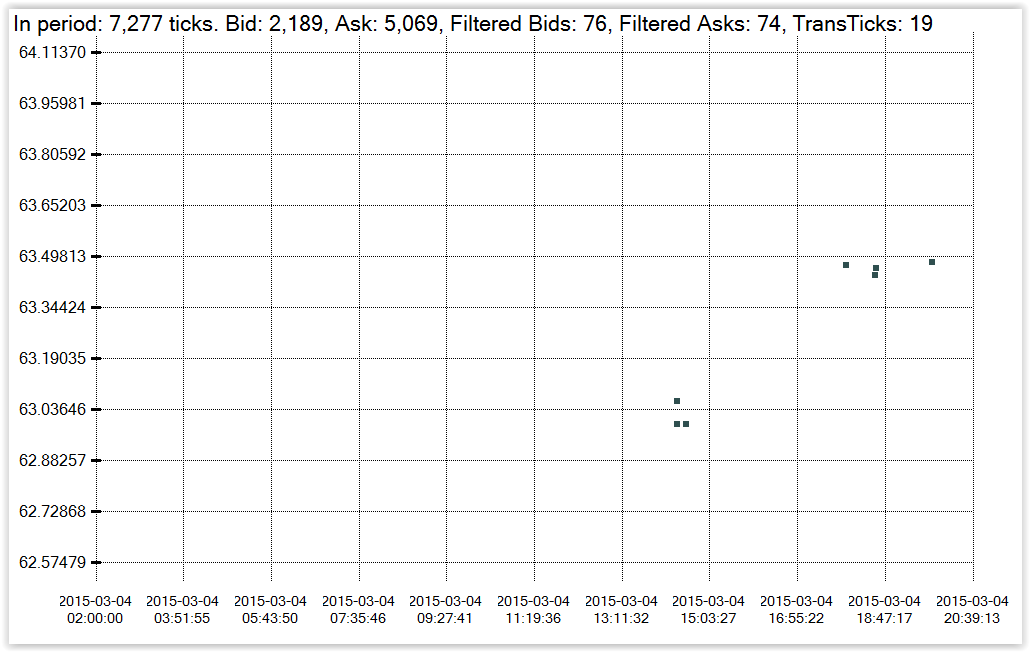
\includegraphics[width=0.8\textwidth]{../wykresy/cottonTickH.PNG}
    \caption{Transactions data for Cotton March Future Contract.}
    \label{fig:esh}
\end{figure}

\end{frame}

\begin{frame}{No transactions does not mean no activity.}

\begin{figure}
    \centering
    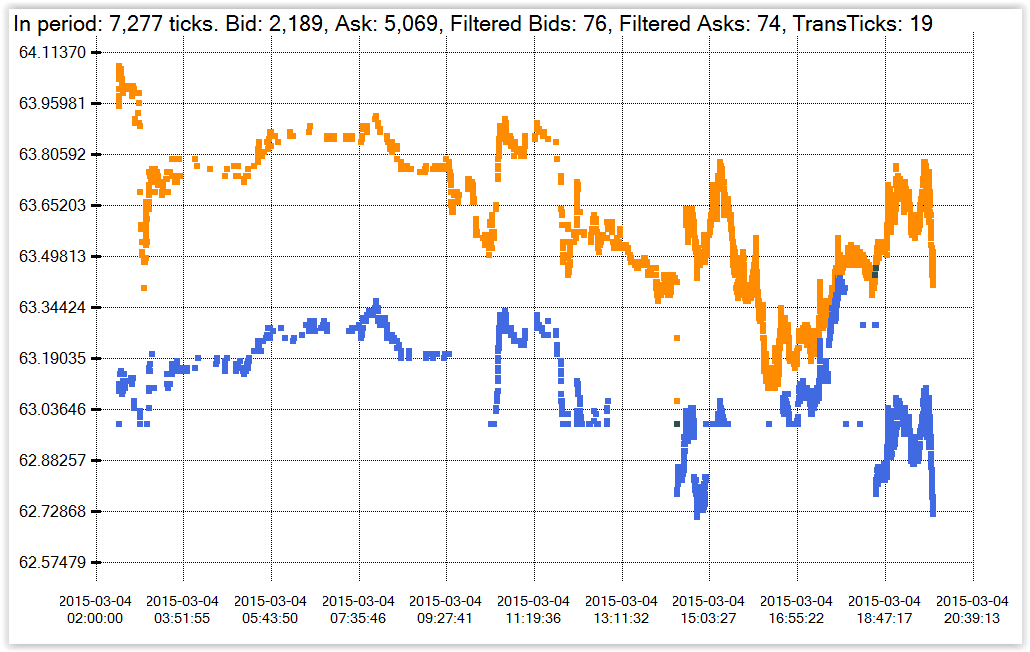
\includegraphics[width=0.8\textwidth]{../wykresy/cottonOrderH.PNG}
    \caption{Activity on order book for Cotton March Future Contract.}
    \label{fig:esh}
\end{figure}

\end{frame}




\section{Empirical evidence on presence of outliers in high-frequency financial data}

\begin{frame}{Empirical evidence on presence of outliers in high-frequency financial data}

\begin{figure}
    \centering
    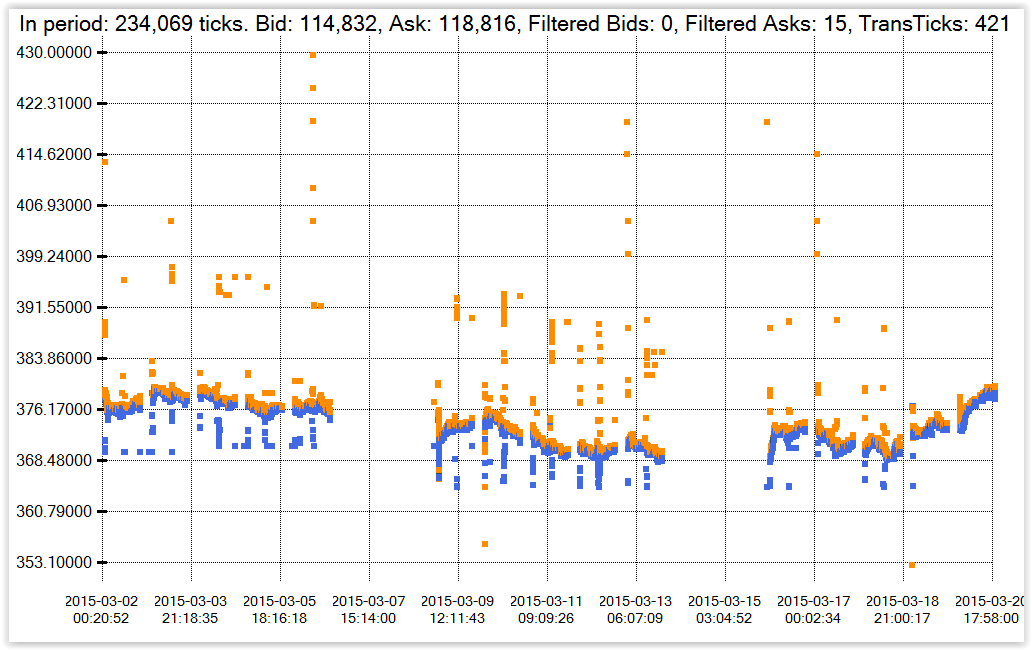
\includegraphics[width=1\textwidth]{../wykresy/fsgj15.PNG}
\end{figure}

\end{frame}


\begin{frame}{"Outliers path" in HFFD}
    
\begin{figure}
    \centering
    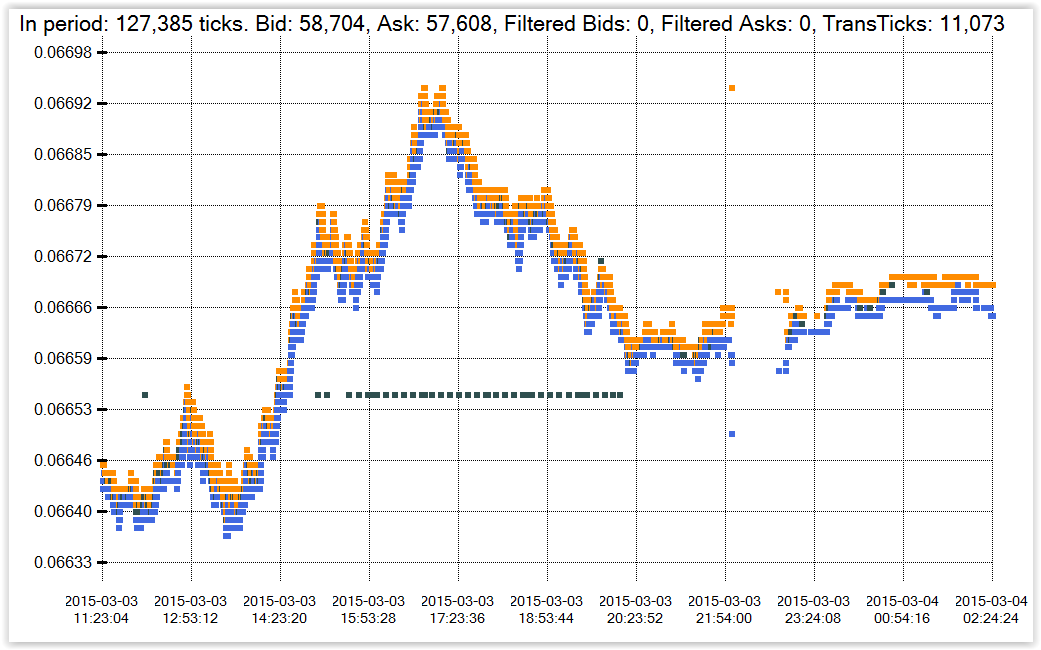
\includegraphics[width=1\textwidth]{../wykresy/f6mh15.PNG}
\end{figure}

\end{frame}

\section{Filter for high frequency financial data}


\begin{frame}{Filter for HFFD - overview}

Main assumptions:

\begin{itemize}
\item Deterministic - results of such filtering should be consistent between backtest.
\item Very fast - it has to deal with large amount of data, possibly tens of thousands per second.
\item Market specific - it should take advantage of special conditions related to a given market while staying fool-proof against large price jumps or data discontinuity. 
\end{itemize}

\end{frame}

\begin{frame}{Filter for HFFD - notation:}
\small
\begin{itemize}
\item \ts - current timestamp.
\item \tsl - timestamp for last tick\footnote{Tick - the best bid/ask change}.
\item \Spt  - spread in time \ts (Spread - difference between Ask and Bid).
\item \MSpc - mean spread in time \ts, before update.
\item \MSpn - mean spread in time \ts, after update of a new observation.
\item \MSpo - mean spread in time \tsl, after update.
\end{itemize}

Parameters:
\begin{itemize}
\item $minSpread$ - minimal spread for instrument.
\item $SprMulti$ - spread multiplier.
\item $\phi_{min}$,$\phi_{max}$ - lower and upper boundaries of the impact of new observation on the value of spread average.
\item $rmMulti$ - value used to update spread when new observation is rejected. It prevents against jamming\footnote{A situation in which all subsequent observation are rejected}.
\end{itemize}

\end{frame}

\begin{frame}{Filter for HFFD - pseudocode}
\small
\begin{algorithm}[H]
\KwData{\\
BidPrice - new best bid.\\
time - tick's timestamp.}
\KwResult{Logical value - false means that current value will be rejected.}

\Spt = AskPrice - BidPrice; \tcc*[r]{AskPrice is a last, not rejected Ask.}



\label{War1}\If{$\Spt \leq SprMulti \cdot \MSpc$ or \\ 
\label{War2}$BidPrice \leq AskPrice + CrossRange$ }
{
\Spt = lastDelAsk - BidPrice; \tcc*[r]{lastDelAsk is a last rejected Ask price.}

	\If{$\Spt \leq SprMulti \cdot \MSpc$ or \\ 
	$BidPrice \leq lastDelAsk + CrossRange$}
	{
		lastDelBid = BidPrice\\
		AskPrice = AskPrice + RmVal\\


	\Return{False}
	
	}
	
AskPrice = lastDelBid
	
}
\Return{True}

\caption{Filter for Bid price\label{FiltrBID}}
\end{algorithm}

\end{frame}

\begin{frame}{Filter for HFFD - pseudocode}

\begin{algorithm}[H]

\eIf{TickAccepted}
{ $\Delta t = t - lastTime$\\
$\phi = exp(\Delta t / \lambda)$\\
$\phi = max(\phi, \phi_{min})$\\
$\phi = min(\phi, \phi_{max})$ \\ 
$\MSpn = \phi \cdot \MSpc + (1 - \phi) \Spt$
}
{
$\MSpn = \MSpc + RmMulti \cdot \MSpc$\\
}

\caption{\MSpn update\label{FiltrUpdate}}
\end{algorithm}

\end{frame}

\begin{frame}{Filtering results.}

\begin{figure}
    \centering
    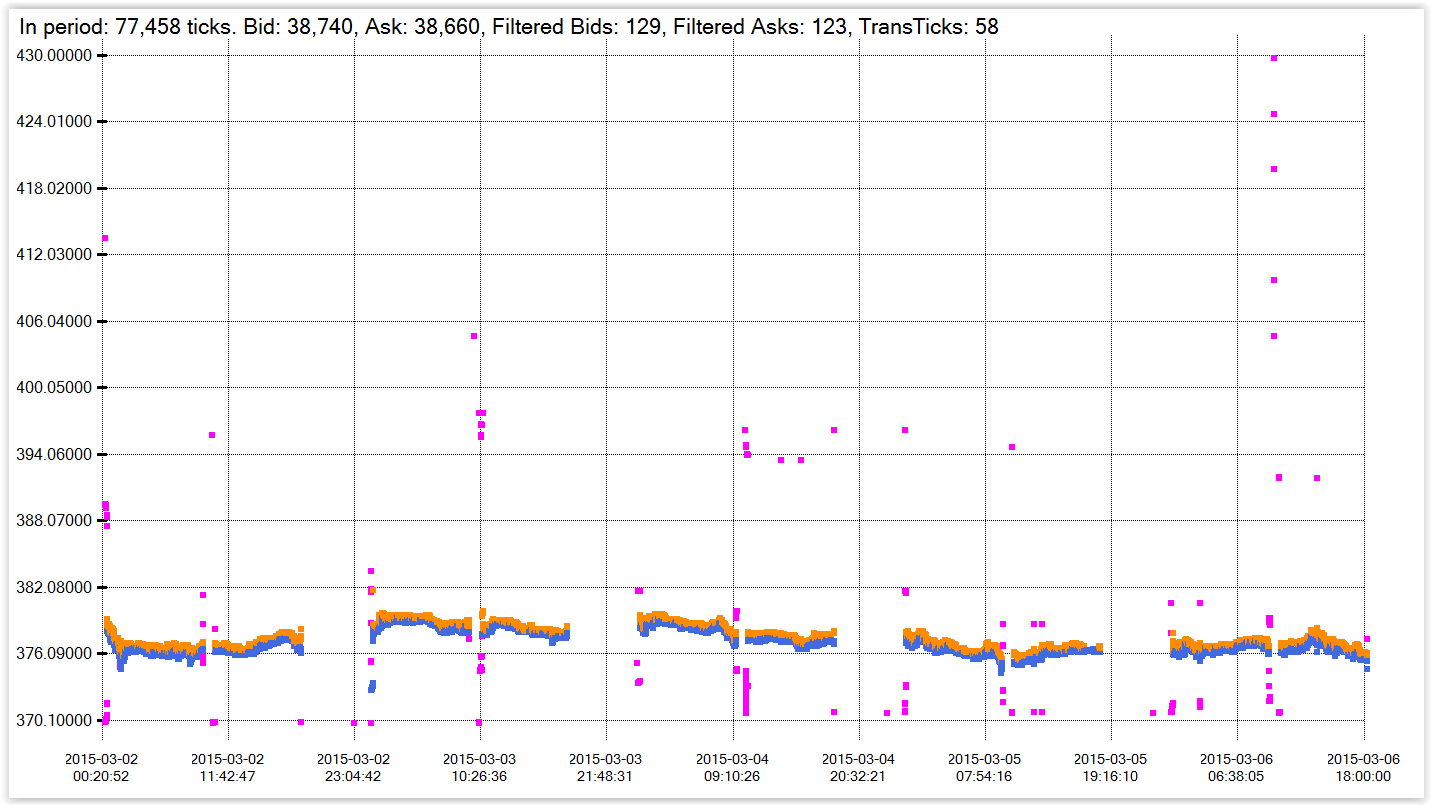
\includegraphics[width=1\textwidth]{../wykresy/sggood.PNG}
\end{figure}

\end{frame}


\begin{frame}{Filtering results.}

\begin{figure}
    \centering
    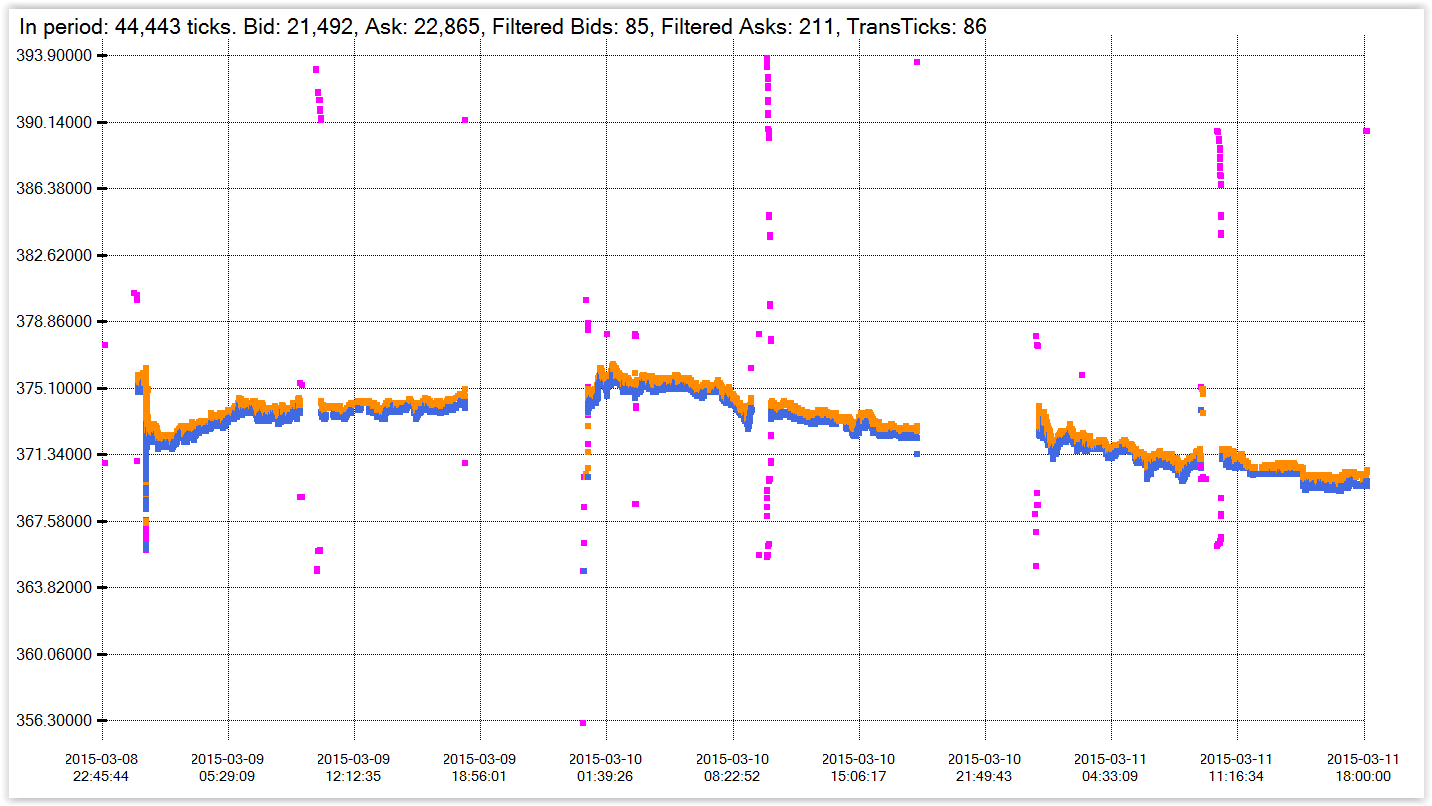
\includegraphics[width=1\textwidth]{../wykresy/sgbadgood.PNG}
\end{figure}

\end{frame}

\begin{frame}{Filtering results - paths of outliers.}

\begin{figure}
    \centering
    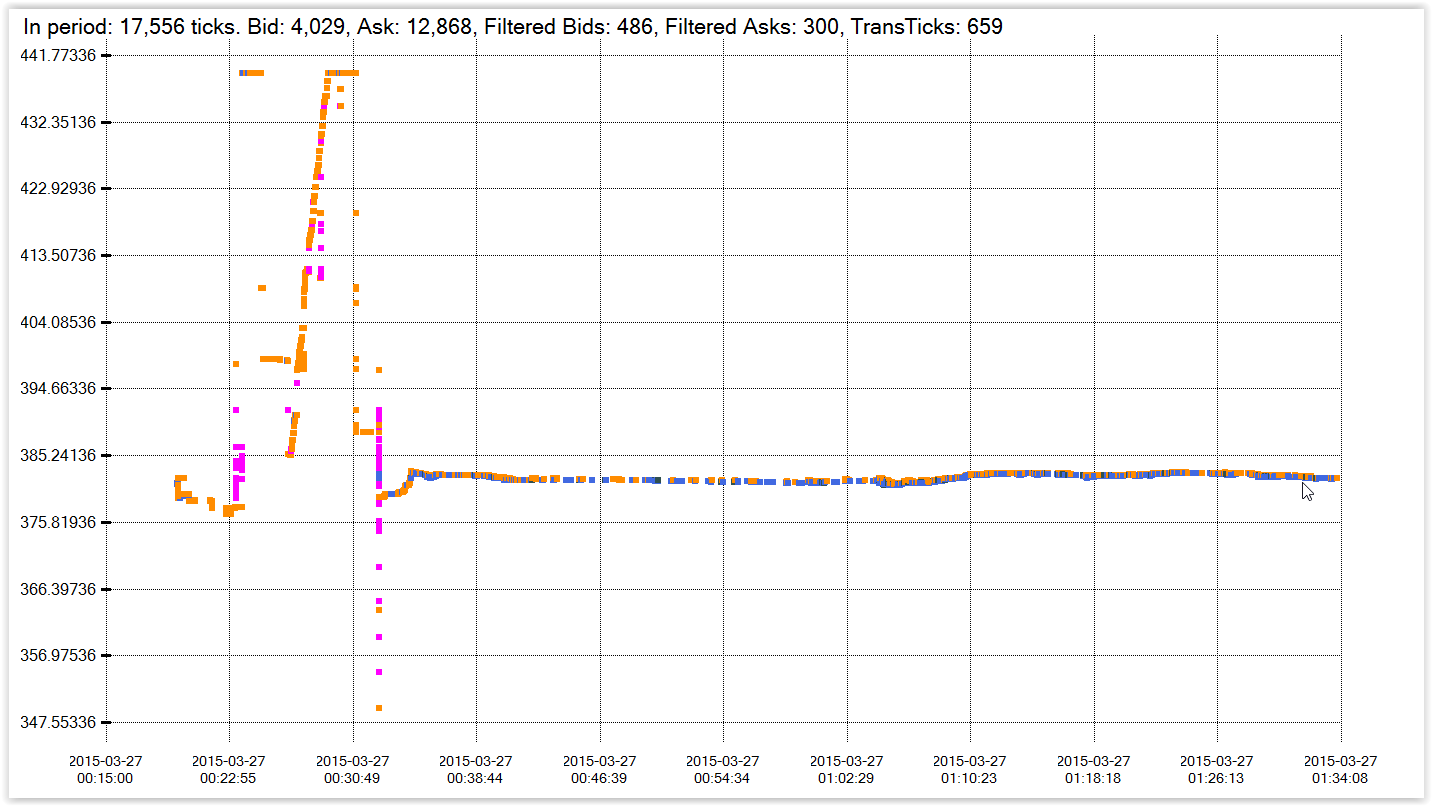
\includegraphics[width=1\textwidth]{../wykresy/pathsgj.PNG}
\end{figure}

\end{frame}

\begin{frame}{Bibliography}
\begin{itemize}
\item W.N. Venables and B.D. Ripley. \emph{Modern applied statistics with S}. New York: Springer, 2002
\item R. Gençay, M. Dacorogna, U. A. Muller, O. Pictet, R. Olsen. \emph{An Introduction to High-Frequency Finance}. Academic Press, 2001
\item  R. F. Engle and J. R. Russel. \emph{Analysis of High Frequency Financial Data} in Handbook of Financial Econometrics. North-Holland, 2004
\item T. H. Falkenberry. \emph{High Frequency Data Filtering}.  Tick Data, white paper, 2002
\end{itemize}


\end{frame}


\end{document}
